% Characterizing Floating-Point Validation Rules for Tensor Superoptimization
% Rev. 5a: consolidation per review 5; two-criterion envelopes (E6); protocol taxonomy.
% Single file; pdflatex on Overleaf.
\documentclass[twocolumn,10pt]{article}
\usepackage[margin=0.9in,columnsep=0.28in]{geometry}
\usepackage{newtxtext,newtxmath}
\usepackage{booktabs}
\usepackage{microtype}
\usepackage{tikz}
\usepackage[colorlinks=true,linkcolor=blue,citecolor=blue,urlcolor=blue]{hyperref}

\newcommand{\atol}{\texttt{atol}}
\newcommand{\rtol}{\texttt{rtol}}
\newcommand{\e}[2]{$#1\times10^{#2}$}

\title{Characterizing Floating-Point Validation Rules\\for Tensor Superoptimization}
\author{Ayaan Faisal\\Rutgers University}
\date{Rev.\ 5a, August 14, 2026}

\begin{document}
\maketitle

\begin{abstract}
Recent tensor superoptimizers specify their semantic verification in detail
while incompletely specifying the empirical floating-point checks applied to
generated implementations. Axon states an elementwise rule,
$|g_i-b_i|\le\atol+\rtol\,|b_i|$ at $\rtol=\atol=10^{-4}$ on FP32; Mirage
describes floating-point filtering without threshold or protocol; Prism
reports random equivalence testing but does not state its numerical
criterion. We characterize a fully specified representative rule and show
that its verdict depends materially on contraction length and output
multiplicity, input scale and distribution, reference implementation,
precision, tolerance constants, and sampling protocol, including the
cross-draw aggregation rule. On our PyTorch/Ampere backend, a
real-equivalent tiled matmul reaches substantial rejection rates at
contraction widths used by deployed 7B-class models ($0/100$ draws at
$K{=}2048$, $48/100$ [38--58\%] at $K{=}4096$, $100/100$ [96--100\%] at
$K{=}11008$ at unit scale; onset near $K{=}1024$ under scale-matched
gaussian inputs at $\sigma$ 2.67). An exact analysis of the measured corpus
shows no nonnegative mixed absolute-relative tolerance with $\rtol\le100$
separates the six real-equivalent rewrites from eighteen injected bugs
under either cross-draw quantifier, while a real eps-placement bug evades
every recorded draw at the published constant. Two plausible references
reverse the direction of oracle-relative accuracy for the same candidate,
and a sequential reference magnifies the difference to $15\times$. Repeated
draws expose per-draw rejection rates ($14/100$ [9--22\%]) that
single-input testing misses. Real-activation FP32 cells pass everywhere
measured. These results do not demonstrate failures in the measured
systems; they identify the protocol coordinates that must be stated for
empirical numerical validation to be reproducible and interpretable.
\end{abstract}

\section{Introduction}

A kernel autotuner tunes a fixed computation against a template that pins
semantics; one reference validates every candidate. A superoptimizer
searches program structure across millions of candidates, and the search
selects for whatever passes the acceptance rule. Mirage~\cite{mirage},
Prism~\cite{prism}, and Axon~\cite{axon} verify candidate equivalence over
exact or idealized arithmetic (Section~\ref{sec:background}) and close the
distance to the compiled floating-point kernel with a sampled comparison
against a reference implementation. Axon and Mirage state this limitation; Prism reports random equivalence
testing without a stated criterion and does not otherwise discuss
floating-point behavior. None fully specifies the reference, threshold, draw protocol, and
precision scope together, so a reader cannot compute what the check
accepts or rejects.

The organizing observation of this study is that a floating-point
validation verdict is not determined by a tolerance pair. It is determined
by a protocol with several independent coordinates: the reference
implementation, the precision, the input distribution and scale, the
per-element comparison rule, the within-tensor aggregation (one violating
element rejects the tensor), the number of independent draws, and the
cross-draw aggregation rule. Our measurements show each coordinate is
load-bearing: changing one, holding the others fixed, changes the verdict.
The findings map onto the coordinates directly: F1 (contraction length,
output multiplicity, input scale, within-tensor aggregation), F2 (tolerance
constants and cross-draw quantifier), F3 (reference implementation), F4
(draw count and cross-draw aggregation), F5 (precision), F6--F7 (input
distribution beyond scale).

Two failure directions are measured on the same rule at the same tolerance:
rejection of rewrites that are algebraic identities over the reals, and
acceptance of injected bugs. The question is not whether any system has
shipped a wrong kernel; we find no evidence of that.

Scope, stated first: we characterize the rule, not the systems' outputs.
The rewrites are PyTorch reimplementations of transformations these systems
accept, run on an Ampere GPU and an Apple M3 with TF32 disabled. No kernel
emitted by Mirage, Prism, or Axon is executed; Axon's deployment target
(Trainium/NKI) differs from our backend in accumulation and lowering, and
FPRev~\cite{fprev} and FTTN~\cite{fttn} document that accumulation order
and extra-precision behavior vary across real libraries and accelerators
and are largely unspecified. Findings transfer to the extent the rule, not
the backend, drives them; Section~\ref{sec:threats} marks which findings
the caveat touches.

A note on labels, following the distinction this study itself surfaces:
``valid'' below means equivalent over the reals, and ``bug'' means
inequivalent over the reals. Real-equivalence is not numerical
acceptability. A real identity can be numerically unstable, and a semantic
bug can be numerically negligible on a given input domain; our corpus
contains both cases, and Section~\ref{sec:findings} keeps the two axes
separate: semantic class is fixed by construction, numerical quality is
measured against a float64 oracle.

Contributions:
\begin{enumerate}
\item A two-class corpus: six real-equivalent rewrites with per-system
provenance (identities established symbolically; implementations validated
to \e{3.5}{-15} against a 50-digit-validated float64 oracle), and eighteen
injected bugs across six classes whose float64 divergences span \e{4.1}{-6}
to \e{8.2}{-1}, sixteen of which form the frontier's severity continuum.
\item An instrument that reports, per cell, the reference's oracle error
(floor), the candidate's oracle error (total), their disagreement
(differential, what the rule tests), the direction ratio total/floor with
absolute errors alongside, and the rule's verdict under three reference
implementations.
\item A tolerance-frontier measurement over the full $(\atol,\rtol)$
grid, plus an exact continuum feasibility computation on the recorded
corpus, answering whether observed failures are a calibration problem or
a rule-family problem.
\item An audit trail: pre-registration with dated amendments, predictions
committed before every run (the log records ten falsified by their own
runs), and an errata with four retracted or corrected results of our own.
\end{enumerate}

\section{Background}\label{sec:background}

Mirage restricts search to its Lax fragment and probabilistically verifies
candidate equivalence by evaluation over random finite-field values; the
theorem bounds the probability of accepting a non-equivalent program, and
the implementation runs a single random test with primes stated in the
paper as $p{=}227$ and $q{=}113$, chosen so their product fits in 16-bit
integers, which the authors acknowledge~\cite{mirage}; the released
artifact's constants are 167 and 83 (Appendix~A). Separately, Mirage v3 (\S5.2) states
that floating-point tests filter $\mu$Graphs with ``significant numerical
errors''; threshold, reference, and draw protocol are unstated. Prism
reasons over roughly 70 hand-written axioms in an e-graph; the axioms are
intended to be sound, a formal proof is stated to be beyond scope, and
every generated kernel is subjected to random equivalence testing with no
stated tolerance, in an evaluation that is entirely half-precision; the
paper does not otherwise discuss floating-point behavior~\cite{prism}.
Axon proves equivalence over the reals with Z3 ($1650\times$ faster than
Z3's floating-point theory on its own example) and validates compiled NKI
kernels on Trainium against a reference implementation on random FP32
inputs at $\rtol=\atol=10^{-4}$~\cite{axon}. Axon does not state how many
independent inputs the numerical gate uses; its evaluation separately
reports 100 timing repetitions on random inputs, so the draw count for
correctness may be one, one hundred, or something else. The three
mechanisms also occupy different roles, a candidate-selection gate (Axon),
a post-generation validation check (Prism), and a numerical-stability
filter (Mirage); we measure the shared rule shape, not any one system's
pipeline.

Two structural properties of the rule drive the measurements. It is
\emph{reference-relative}: the target is another floating-point
implementation, not a higher-precision oracle, so the rule cannot observe
which side of a disagreement is more accurate. And it is \emph{mixed
absolute-relative}: \rtol\ scales with each output element, but near zero
the fixed \atol\ is the only protection, while accumulated rounding error
grows with reduction length rather than with the element's own magnitude.

\section{Method}

\paragraph{Valid corpus (registered).} Six (reference, candidate) pairs,
each an algebraic identity over the reals: split reduction, reassociation,
scalar multiplication moved past matmul, LayerNorm two-pass vs.\ fused
one-pass variance, naive vs.\ online softmax, matmul $K$-tiling.
Identities hold symbolically; the float64 check (18 cells within
\e{6}{-16} to \e{3.5}{-15}) validates the implementations; the float64
oracle is validated against 50-digit \texttt{mpmath} (worst drift
\e{8.2}{-16}) at small shapes and assumed adequate at large ones. A
negative control establishes a nonzero instrument reading.

\paragraph{Mutant corpus (amended, registered before execution).} Six bug
classes, eighteen instances. Four classes parameterize into the sixteen
instances the tolerance frontier sweeps: dropped reduction elements ($j
\in \{1,2,4,8,16,32\}$), dropped contraction columns ($j \in
\{1,2,8,32\}$), Bessel-style divisors ($n{-}j$, $j \in \{1,2,8\}$), and
eps added to the standard deviation instead of the variance (eps in
\e{1}{-5} to \e{1}{-3}). Two gross single-instance classes run in the
detection arm only: a missing online-softmax rescale and a dropped
$K$-tile. The implemented column grid is sparser than the registered
$\{1..32\}$ set; the deviation is recorded in the errata. Float64
divergences span \e{4.1}{-6} (eps placement) to \e{8.2}{-1} (missing
rescale), overlapping the valid corpus's floating-point disagreement
range, which is what makes the discrimination question nondegenerate.

\paragraph{Instrument.} Oracle: the reference computed in float64 on the
same rounded inputs the test-precision run sees, excluding input
quantization. Per cell: floor, total, differential, the direction ratio
total/floor with absolute errors alongside (ratios are unstable as floor
approaches zero), element exceedance fractions, and the rule verdict. An
earlier ratio (differential/floor) was direction-blind and is retired; the
errata records the misreading it caused.

\paragraph{Evidence classes.} Claims below signal their evidence type by
verb. Recorded facts about the measured corpus use ``observed,'' ``on all
recorded draws,'' ``on the measured corpus,'' and may be stated exactly.
Statistical estimates carry rates with Wilson 95\% intervals and
``estimated'' or ``consistent with.'' Generalizations beyond the backend,
model, or corpus use ``on our backend,'' ``suggests,'' or ``may
transfer,'' and carry scope qualifiers.

\paragraph{Protocol labels.} Analyses are marked \emph{registered} (in the
original claim), \emph{amended} (registered by dated amendment before
execution: the mutant arm, the tolerance frontier, the $K$ extension, the
decomposition, the library reference, the C1--C3 pass, the separability
computations E5--E6, and the grid completion E7), or \emph{exploratory}
(single-draw sweeps that motivated later registered runs). Predictions
precede every run in the committed log.

\section{Findings}\label{sec:findings}

\paragraph{F1. Rejection of the valid tiled matmul reaches contraction
widths used by deployed models under our pinned test geometry.} The
mechanism, backend-independent in kind: near-zero output elements lose the
relative allowance, accumulated rounding disagreement grows with reduction
length, and the any-element aggregation turns rare element violations into
tensor rejection (in diagnosed failing draws, one element in 4096, its
magnitude $750\times$ below the tensor median). The measured onset,
backend-specific: on our PyTorch/Ampere--M3 backend under the literal
elementwise rule at $M{=}N{=}64$, 100 draws per cell
(Table~\ref{tab:ksweep}, Figure~\ref{fig:kscale}), $K{=}4096$ and 11008 are
the projection and MLP contraction widths of Llama-2-7B~\cite{llama2}; the
$\sigma$ column uses scale-matched gaussian inputs ($\sigma=2.67$, matching
the measured activation scale), and the onset falls roughly fourfold from
its unit-scale position. Rejection is non-decreasing along both axes (the
$\sigma$ axis at $K{=}512$ reads 0, 0, 1, 16, 74 per 100 at $\sigma$ from
0.5 to 4.0). Tensor-scale relative disagreement stays near $10^{-6}$
throughout, so no tensor-scale relative statistic predicts the verdict. A
simple independence approximation over the rule's any-element quantifier,
from the measured per-element exceedance of \e{3.42}{-5} at $K{=}512$,
gives 13.1\%, consistent with the observed [9--22\%]; dependence among
output elements is not established either way. A correction preserved from
an earlier revision: a prior ``fails at $K{=}2048$'' verdict came from
comparing maximum absolute difference against \atol\ alone, ignoring the
\rtol\ term, the same quantity confusion this paper studies; the errata
records it.

\begin{table}[t]
\centering
\begin{tabular}{@{}rllll@{}}
\toprule
$K$ & \multicolumn{2}{l}{unit scale} & \multicolumn{2}{l}{$\sigma=2.67$} \\
\midrule
512   & 0/100   & [0, 4]    & 11/100  & [6, 19] \\
1024  & 0/100   & [0, 4]    & 69/100  & [59, 77] \\
2048  & 0/100   & [0, 4]    & 100/100 & [96, 100] \\
4096  & 48/100  & [38, 58]  & 100/100 & [96, 100] \\
11008 & 100/100 & [96, 100] & 100/100 & [96, 100] \\
\bottomrule
\end{tabular}
\caption{The valid $K$-tiled matmul under the literal elementwise rule,
$M{=}N{=}64$, fp32, 100 draws per cell, Wilson 95\% CIs in percent.}
\label{tab:ksweep}
\end{table}

\begin{figure}[t]
\centering
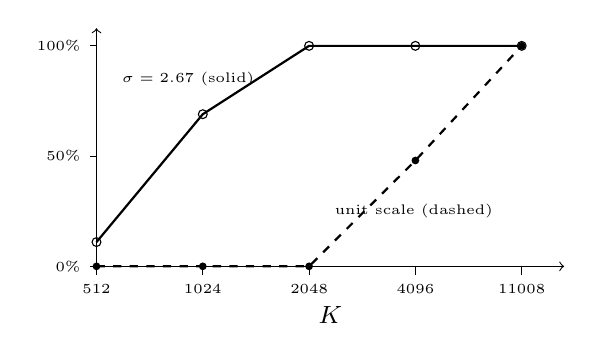
\begin{tikzpicture}[x=1.35cm,y=0.028cm]
\draw[->] (0,0) -- (4.4,0);
\draw[->] (0,0) -- (0,108);
\foreach \y in {0,50,100} { \draw (0,\y) -- (-0.06,\y)
  node[left,font=\tiny] {\y\%}; }
\foreach \i/\k in {0/512,1/1024,2/2048,3/4096,4/11008} {
  \draw (\i,0) -- (\i,-4) node[below,font=\tiny] {\k}; }
\draw[thick,dashed] (0,0) -- (1,0) -- (2,0) -- (3,48) -- (4,100);
\foreach \i/\y in {0/0,1/0,2/0,3/48,4/100} { \fill (\i,\y) circle (1.4pt); }
\draw[thick] (0,11) -- (1,69) -- (2,100) -- (3,100) -- (4,100);
\foreach \i/\y in {0/11,1/69,2/100,3/100,4/100} {
  \draw (\i,\y) circle (1.6pt); }
\node[right,font=\tiny] at (2.15,25) {unit scale (dashed)};
\node[right,font=\tiny] at (0.15,85) {$\sigma=2.67$ (solid)};
\node[below,font=\small] at (2.2,-14) {$K$};
\end{tikzpicture}
\caption{Rejection rate of the valid $K$-tiled matmul against contraction
width, 100 draws per point, under unit-scale and scale-matched gaussian
inputs. The onset shifts roughly fourfold with input scale.}
\label{fig:kscale}
\end{figure}

\paragraph{F2. No mixed absolute-relative tolerance separates the measured
corpus, under either cross-draw quantifier.} On the recorded per-element
errors, with $A_V(r)$ the smallest \atol\ accepting every valid draw at
relative tolerance $r$: under criterion \textsc{every} (each mutant draw
rejected), no $(\atol \ge 0, \rtol \le 100)$ separates; all 400
inter-sample intervals carry a convexity certificate and the supremum of
the separation gap is $-3.5\times10^{-5}$. Under criterion \textsc{some}
(each mutant caught on at least one recorded draw), the result is the
same, with the gap narrowing to $-4.0\times10^{-6}$: the weaker quantifier
comes within 4 millionths of admitting a separator but never does. The
cross-draw aggregation rule, which no source paper states, moves the
separation margin ninefold. On the 64-point grid
(Figure~\ref{fig:frontier}), the minimum total error is a three-point
plateau, $(10^{-4},10^{-4})$, $(10^{-4},10^{-3})$, $(10^{-4},10^{-2})$, at
0\% valid rejection (unit scale) plus a 6.25\% mutant-instance miss
fraction, meaning 1 of the 16 frontier instances, equivalently 50 of 800
mutant draws, all from the eps-$10^{-5}$ bug; this fraction describes the
constructed corpus, not any candidate population. Axon's published
constant lies on the plateau and \atol\ is the binding coordinate, the
near-zero-element mechanism restated. The evading bug's severity is
input-dependent (it grows as row variance approaches eps), so detection
statements hold at the measured input statistics; an oracle-referenced
check with a condition-aware budget \emph{could} see it where the sampled
rule cannot, though whether a principled budget resolves \e{4.1}{-6} at
these statistics is not demonstrated. Under scale-matched gaussian inputs
at $\sigma$ 2.67 the picture is unchanged: five gross mutants at $100/100$
detection, the eps bug evading all 100 draws, its divergence shrinking to
\e{2.46}{-6} as the registered mechanism predicts.

\begin{figure}[t]
\centering
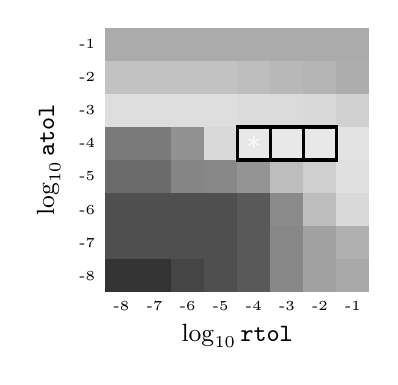
\begin{tikzpicture}[x=0.42cm,y=0.42cm]
\fill[black!80] (0,0) rectangle (1,1);
\fill[black!80] (1,0) rectangle (2,1);
\fill[black!73] (2,0) rectangle (3,1);
\fill[black!69] (3,0) rectangle (4,1);
\fill[black!65] (4,0) rectangle (5,1);
\fill[black!47] (5,0) rectangle (6,1);
\fill[black!37] (6,0) rectangle (7,1);
\fill[black!34] (7,0) rectangle (8,1);
\fill[black!69] (0,1) rectangle (1,2);
\fill[black!69] (1,1) rectangle (2,2);
\fill[black!69] (2,1) rectangle (3,2);
\fill[black!69] (3,1) rectangle (4,2);
\fill[black!65] (4,1) rectangle (5,2);
\fill[black!47] (5,1) rectangle (6,2);
\fill[black!37] (6,1) rectangle (7,2);
\fill[black!31] (7,1) rectangle (8,2);
\fill[black!69] (0,2) rectangle (1,3);
\fill[black!69] (1,2) rectangle (2,3);
\fill[black!69] (2,2) rectangle (3,3);
\fill[black!69] (3,2) rectangle (4,3);
\fill[black!65] (4,2) rectangle (5,3);
\fill[black!46] (5,2) rectangle (6,3);
\fill[black!26] (6,2) rectangle (7,3);
\fill[black!15] (7,2) rectangle (8,3);
\fill[black!58] (0,3) rectangle (1,4);
\fill[black!58] (1,3) rectangle (2,4);
\fill[black!48] (2,3) rectangle (3,4);
\fill[black!47] (3,3) rectangle (4,4);
\fill[black!42] (4,3) rectangle (5,4);
\fill[black!26] (5,3) rectangle (6,4);
\fill[black!19] (6,3) rectangle (7,4);
\fill[black!12] (7,3) rectangle (8,4);
\fill[black!52] (0,4) rectangle (1,5);
\fill[black!52] (1,4) rectangle (2,5);
\fill[black!43] (2,4) rectangle (3,5);
\fill[black!15] (3,4) rectangle (4,5);
\fill[black!9] (4,4) rectangle (5,5);
\fill[black!9] (5,4) rectangle (6,5);
\fill[black!9] (6,4) rectangle (7,5);
\fill[black!11] (7,4) rectangle (8,5);
\fill[black!13] (0,5) rectangle (1,6);
\fill[black!13] (1,5) rectangle (2,6);
\fill[black!13] (2,5) rectangle (3,6);
\fill[black!13] (3,5) rectangle (4,6);
\fill[black!14] (4,5) rectangle (5,6);
\fill[black!14] (5,5) rectangle (6,6);
\fill[black!15] (6,5) rectangle (7,6);
\fill[black!18] (7,5) rectangle (8,6);
\fill[black!24] (0,6) rectangle (1,7);
\fill[black!24] (1,6) rectangle (2,7);
\fill[black!24] (2,6) rectangle (3,7);
\fill[black!24] (3,6) rectangle (4,7);
\fill[black!26] (4,6) rectangle (5,7);
\fill[black!28] (5,6) rectangle (6,7);
\fill[black!29] (6,6) rectangle (7,7);
\fill[black!32] (7,6) rectangle (8,7);
\fill[black!33] (0,7) rectangle (1,8);
\fill[black!33] (1,7) rectangle (2,8);
\fill[black!33] (2,7) rectangle (3,8);
\fill[black!33] (3,7) rectangle (4,8);
\fill[black!33] (4,7) rectangle (5,8);
\fill[black!33] (5,7) rectangle (6,8);
\fill[black!33] (6,7) rectangle (7,8);
\fill[black!33] (7,7) rectangle (8,8);
\draw[very thick] (4,4) rectangle (5,5);\draw[very thick] (5,4) rectangle (6,5);\draw[very thick] (6,4) rectangle (7,5);
\node[white] at (4.5,4.5) {$\ast$};
\node[below,font=\tiny] at (0.5,0) {-8};\node[below,font=\tiny] at (1.5,0) {-7};\node[below,font=\tiny] at (2.5,0) {-6};\node[below,font=\tiny] at (3.5,0) {-5};\node[below,font=\tiny] at (4.5,0) {-4};\node[below,font=\tiny] at (5.5,0) {-3};\node[below,font=\tiny] at (6.5,0) {-2};\node[below,font=\tiny] at (7.5,0) {-1};\node[left,font=\tiny] at (0,0.5) {-8};\node[left,font=\tiny] at (0,1.5) {-7};\node[left,font=\tiny] at (0,2.5) {-6};\node[left,font=\tiny] at (0,3.5) {-5};\node[left,font=\tiny] at (0,4.5) {-4};\node[left,font=\tiny] at (0,5.5) {-3};\node[left,font=\tiny] at (0,6.5) {-2};\node[left,font=\tiny] at (0,7.5) {-1};
\node[below=8pt,font=\small] at (4,0) {$\log_{10}\rtol$};
\node[rotate=90,font=\small] at (-1.7,4) {$\log_{10}\atol$};
\end{tikzpicture}
\caption{Total corpus error (valid-rewrite rejection fraction plus
mutant corpus miss fraction) over the 64-point $(\atol,\rtol)$ grid,
50 draws per program; darker is worse. Outlined cells: the optimum
plateau (0\% valid rejection, 6.25\% corpus miss fraction). Star:
Axon's published constant. The exact feasibility computation (E5)
extends the no-separator result to the continuum for $\rtol\le100$.}
\label{fig:frontier}
\end{figure}

\paragraph{F3. Two plausible references reverse the direction of the
accuracy comparison; a sequential reference magnifies it to $15\times$.}
Observed on the measured corpus at fp16, for the same online-softmax
candidate (absolute oracle errors in parentheses): against the strided-tree
reference the candidate is $1.6\times$ closer to the oracle than its
reference (\e{6.0}{-4} vs \e{9.7}{-4}) and the rule passes it on $98/100$
draws [93--99\%]; against \texttt{torch.sum} it is $1.6\times$ farther
(\e{6.0}{-4} vs \e{3.7}{-4}) and the rule passes it on $99/100$
[95--100\%]; against sequential accumulation it is $15\times$ closer
(\e{6.0}{-4} vs \e{8.9}{-3}) and the rule fails it on $100/100$
[96--100\%]. At bf16 the ratios are 1.92, 2.14, and 0.02, and the rule
fails all three on $100/100$. The mean floors order seq $>$ tree $>$
\texttt{torch.sum}, but the per-draw ordering holds on only $80/100$
(fp16) and $85/100$ (bf16) draws: the ranking of references is itself
draw-dependent. \texttt{torch.sum}'s smaller floor is consistent with a
different internal accumulation strategy, which we do not characterize
here; FPRev independently demonstrates that such accumulation orders are
implementation properties that are often undocumented~\cite{fprev}.
Reference-relative validation penalizes differing rather than being wrong:
the cells where our two gate definitions disagree are exactly the cells
where the candidate is closer to the oracle than its reference.

\paragraph{F4. Detection is a rate, and neither the draw count nor the
cross-draw rule is stated by any source paper.} Observed: the valid
$K{=}512$ tiling trips the rule on $14/100$ draws [9--22\%] under
scale-matched gaussian inputs ($\sigma=2.67$) and $0/100$ at unit scale
(upper bound 4\%); an independent registered replication reads $16/100$
[10--24\%]. Our own exploratory single-draw sweep missed the failure; the
registered repeated-draw run caught it. Two aggregation questions govern
what such rates mean. Within a tensor, Axon's rule is elementwise and
unambiguous: one violating element rejects the tensor. Across random
inputs, everything is unstated: the number of draws, whether a candidate
must pass all of them, and how errors aggregate. As hypothetical
consequences under IID draws and an all-draws-must-pass rule, not
measurements of any system: a valid rewrite with a 14\% per-draw rejection
rate survives 20 draws with probability near $0.86^{20} \approx 4.9\%$;
and a $0/100$ observation is consistent both with a true catch probability
of zero (more draws never help) and with a rate at its 3.7\% upper bound,
where 100 draws would catch the bug with probability near 97.7\%. A
reported draw count without its cross-draw aggregation rule is still not
enough to reproduce a validator.

\paragraph{F5. An FP32-class fixed tolerance does not transfer to reduced
precision.} An untransformed matmul deviates from exact arithmetic on its own inputs
(scale-relative: maximum absolute difference over maximum oracle
magnitude) by \e{3.95}{-4} at fp16 and \e{3.10}{-3} at bf16, at or above
the $10^{-4}$ scale, and all 36 reduced-precision cells fail a
$10^{-4}$-class rule. The direction ratio shows the failures are dominated
by reference and precision error rather than by the rewrites: against the
sequential reference the reordering candidates are $3\times$ to $73\times$
closer to the oracle than the reference they fail against ($8\times$ to
$62\times$ at the mlp shapes). Axon scopes its constant to FP32
explicitly; Prism's benchmarks are half-precision with no stated
threshold; so this finding is a constraint on any future stated rule, not
evidence that a system's actual criterion fails.

\paragraph{F6. Real activations are benign in this model.} Every
real-activation cell passes at fp32 with at least $10\times$ headroom,
including post-LayerNorm row sums at condition number 368{,}927,
$400\times$ beyond unit-gaussian reach (condition rose $400\times$, error
rose $11\times$). The fused-variance hazard does not materialize because
the captured residual stream is empirically near zero-mean per row
(cancellation statistic at most 0.016), an observation about this 6-layer
pre-norm model, not an architectural guarantee. The evidence base is one
small character-level model and one batch; broader pretrained-model
coverage is the highest-value extension.

\paragraph{F7. Inputs that force valid-corpus failures are far outside the
observed activation distribution.} Constructed cancellation inputs trip
the rule on every draw, but their median row condition number is
\e{4.5}{6} against 42.8 for real rows ($10.4\sigma$ on a log scale), and
the elementwise violations are near $2\times$ tolerance. Online softmax is
immune under every strategy measured; it is also the pair the verifiers
handle worst, by our inference from their mechanisms: its running
\texttt{max} is not a Lax operator, so Mirage partitions around it, and
Axon's uninterpreted $\exp$ blocks the rescale identity; neither paper
classifies the transformation itself. Exceptional regimes (NaN, Inf,
subnormals, overflow) are not covered by our gaussian and activation
inputs and remain open.

\section{Threats to validity}\label{sec:threats}

\paragraph{Backend and reimplementation (F1--F5).} No emitted kernel from
any system is executed; PyTorch reimplementations on Ampere/M3 stand in,
while FPRev and FTTN document that real accumulation orders and
extra-precision behavior vary across libraries and accelerators. The
frontier and $K$ results characterize the rule on our backend; magnitudes
on Trainium or cuBLAS paths may differ.

\paragraph{Mutant severity is input-dependent (F2).} Detection rates are
statements at the stated input statistics; the evading bug grows as
variance approaches eps.

\paragraph{Reference coverage (F3).} Three references (sequential,
strided-tree, \texttt{torch.sum}) bound the effect on one backend;
production references are undocumented multiway trees.

\paragraph{One model, one batch (F6).} A pretrained-transformer activation
corpus across layers and batches is the single most valuable missing
dataset.

\paragraph{Oracle and ratios.} The float64 oracle is validated at small
shapes; direction ratios are reported with absolute errors because they
are unstable as floor approaches zero. Exploratory single-draw cells exist
and are labeled; headline claims rest on registered repeated-draw runs.

\paragraph{Selection amplification (not measured).} A validator inside a
superoptimizer is queried repeatedly by an adaptive candidate-generation
process, so rare misses may be amplified by selection. Quantifying that
requires a candidate distribution or an actual search loop; it is the
natural next registered experiment, and the mutant-instance miss fraction above is
not an estimate of any candidate-population miss probability.

\section{Implications}

\paragraph{For Axon.} Its constant is, on our corpus, on the optimum plateau of its rule family
(F2), and the family cannot separate the classes under either cross-draw
quantifier;
its rule's verdict becomes shape-dependent within deployed contraction
widths on our backend, for a system whose proofs are shape-generic (F1). What the measurements support
reporting: the draw count, the reference implementation and its accumulation order,
and a justified error budget appropriate to the operator, shape, and
precision, with accumulation dependence where applicable, of the kind
derived for mixed-precision GEMM by Blanchard et al.~\cite{blanchard} and
Higham and Mary~\cite{highammary}. An oracle
comparison could preserve accuracy-improving candidates (F3); a fixed
reference-relative rule cannot.

\paragraph{For Prism.} Half-precision evaluation with an unstated
threshold sits exactly where F5 shows fixed FP32-class constants do not
transfer; a stated and justified tolerance for its half-precision regime would make
its random testing interpretable.

\paragraph{For Mirage.} The v3 numerical-stability filter is the right
mechanism; stating its threshold, reference, and draw count would make it
the first fully specified floating-point acceptance rule in this
literature.

\paragraph{Method integrity.} Four of our own results were retracted or
corrected during this study: a mischaracterization of Mirage's testing
(stale paper version), a direction-blind metric interpretation refuted by
our own records, an unsupported single-draw attribution, and a $K{=}2048$
rejection verdict produced by comparing a maximum absolute difference
against \atol\ alone, the same quantity confusion this paper criticizes in
tolerance reporting. Every correction moved against our registered claim.
The errata and dated run log are part of the artifact.

\section{Related work}

TASO~\cite{taso} began validation-adjacent practice in tensor
superoptimization, using random-tensor execution to identify
candidate-equivalent graphs before formally verifying substitutions.
TensorRight~\cite{tensorright} develops stronger idealized rewrite
verification; Mirage, Prism, and Axon combine stronger semantic reasoning
with residual empirical validation of generated implementations. TTrace~\cite{ttrace} is the closest adjacent study:
in distributed-training validation it shows fixed \texttt{torch.allclose}
tolerances produce false positives, false negatives, or both, and
replaces them with perturbation-derived dynamic tolerances; our subject
differs (superoptimizer acceptance rules, real-equivalent rewrites and
injected bugs, reference and shape sensitivity), and our envelope analysis
complements its diagnosis by showing no fixed pair separates our corpus
at all. Concurrent 2026 measurements reach
adjacent conclusions on neighboring workloads: fixed-shape small-sample
allclose oracles pass seeded-bug GPU kernels~\cite{illusion}, per-operator
and per-dtype tolerance calibration trades detection against false
positives~\cite{opaware}, and input-generation strategy materially changes
which kernel bugs surface~\cite{testinput}; none studies the
superoptimizer acceptance stage or reference sensitivity. FPRev~\cite{fprev} infers the
undocumented accumulation orders of real libraries and accelerators
(multiway trees on tensor cores), and FTTN~\cite{fttn} shows accelerator
numerical features are under-documented across vendors; both make F3's
reference sensitivity a systems fact rather than a constructed example.
LifeJacket~\cite{lifejacket} and Alive-FP~\cite{alivefp} verify LLVM
floating-point optimizations under actual FP semantics and found real
incorrect optimizations, precedent for evaluating both valid and invalid
transformations; Minotaur~\cite{minotaur} brings formal FP reasoning to
SIMD superoptimization. NNSmith~\cite{nnsmith} treats input generation as
central to exposing compiler bugs, as our scale and distribution findings
do for validation. Herbie~\cite{herbie} rewrites for accuracy, the
direction sensitivity reference-relative rules lack.
FPBench~\cite{fpbench} standardizes accuracy measures for FP tools, the
measurement-definition problem our oracle and metric choices address.
Rounding-error analyses (Goldberg~\cite{goldberg}; Higham~\cite{higham};
SATIRE~\cite{satire}; Blanchard et al.~\cite{blanchard}; Higham and
Mary~\cite{highammary}) derive the accumulation-dependent budgets a
specified rule could use in place of a constant. Mytkowicz et
al.~\cite{wrongdata} showed performance evaluation produces wrong
conclusions from unexamined setup; this paper applies the same
measurement scrutiny to correctness validation.

\section{Conclusion}

A numerical validation result is interpretable only relative to a
specified validation protocol, and the measurements here show that
individual protocol coordinates materially change the verdict: contraction
length and output multiplicity (F1), tolerance constants and the
cross-draw quantifier (F2), reference implementation (F3), draw count
(F4), precision (F5), and input scale and distribution (F1, F6, F7). On
the measured corpus, no nonnegative mixed absolute-relative tolerance with
$\rtol \le 100$ separates real-equivalent rewrites from injected bugs
under either cross-draw semantics. Real-activation FP32 cells passed
everywhere measured, and no evidence indicates any system has shipped an
incorrect kernel.

The constructive conclusion is a reporting standard, not a replacement
validator. A floating-point acceptance result should specify at least:
(1) the reference implementation and its relevant accumulation behavior;
(2) the precision; (3) the input distribution and scale; (4) the
per-element comparison function and constants; (5) the within-tensor
aggregation rule; (6) the number of independent draws; (7) the cross-draw
aggregation rule; and (8) a justification for the numerical error budget
in the operator, shape, and precision regime. This paper does not
prescribe one universal validator; it identifies the information necessary
to make a validator's result reproducible and interpretable, and measures
what remains undetermined when that information is absent.

\paragraph{Artifact.} All measurements reproduce from the public
repository; each experiment runs from one script, raw per-cell records
are committed, and the pre-registration, amendments, run log, and errata
are public. AI tools (Claude) assisted with code, measurements, and
documentation; the developer directed, reviewed, and verified all work,
and no measured number comes from a model.

\section*{Appendix A: implementation observations on the Mirage artifact}

Exploratory; the checklist of Section~8 applied to a released artifact.
Audited: \texttt{mirage-project/mirage} at commit \texttt{5c28cc6}
(2026-07-28) with the \texttt{evaluation} branch cross-checked; method and
positive controls in the repository audit notes. The released
\texttt{superoptimize} path is search, exact finite-field fingerprint
verification, transpilation, then performance-only selection over random
inputs; no floating-point comparison exists at the acceptance stage, so
the tolerance, precision, and input-distribution coordinates are moot
there, while the per-element rule (exact field equality), reference
(input-graph fingerprints), draw count (a single fingerprint evaluation
per candidate, consistent with the paper's acknowledged single test), and
aggregation (all outputs must match) are determined by code. The
numerical-stability filter described in the paper's v3 (\S5.2) is not
locatable in the released search path at these commits; float tolerances
appear only in demos and runtime-kernel tests. The finite-field constants
are \texttt{FP\_P}=167, \texttt{FP\_Q}=83 on both audited branches,
while the paper states $p{=}227$, $q{=}113$; under the paper's per-test
acceptance bound, which scales as $1/q$, the released configuration is
weaker than the stated one by roughly $1.4\times$. These are observations
about the released repository at pinned commits, not about any deployed
system.

\begin{thebibliography}{22}
\bibitem{mirage} M.~Wu et al. Mirage: A Multi-Level Superoptimizer for
Tensor Programs. OSDI 2025. arXiv:2405.05751 (v3).
\bibitem{prism} M.~Wu, X.~Jiang, O.~Padon, Z.~Jia. Prism: Symbolic
Superoptimization of Tensor Programs. arXiv:2604.15272.
\bibitem{axon} A.~Kothari, S.~Zhu, D.~Kroening, C.~Sung. Axon: A
Synthesizing Superoptimizer for Tensor Programs. arXiv:2606.26344.
\bibitem{tensorright} J.~Arora et al. TensorRight: Automated Verification
of Tensor Graph Rewrites. PACMPL 9 (POPL), 2025.
\bibitem{taso} Z.~Jia, O.~Padon, J.~Thomas, T.~Warszawski, M.~Zaharia,
A.~Aiken. TASO: Optimizing Deep Learning Computation with Automatic
Generation of Graph Substitutions. SOSP 2019.
\bibitem{ttrace} Jiang et al. TTrace: Lightweight Error Checking and
Diagnosis for Distributed Training. arXiv:2506.09280.
\bibitem{fprev} Xie et al. Revealing Floating-Point Accumulation Orders in
Software/Hardware Implementations. USENIX ATC 2025. arXiv:2411.00442.
\bibitem{fttn} X.~Li et al. FTTN: Feature-Targeted Testing for Numerical
Properties of NVIDIA and AMD Matrix Accelerators. arXiv:2403.00232.
\bibitem{ruler} C.~Nandi, M.~Willsey, et al. Rewrite Rule Inference Using
Equality Saturation. OOPSLA 2021.
\bibitem{herbie} P.~Panchekha, A.~Sanchez-Stern, J.~R.~Wilcox, Z.~Tatlock.
Automatically Improving Accuracy for Floating Point Expressions. PLDI 2015.
\bibitem{alivefp} D.~Menendez, S.~Nagarakatte, A.~Gupta. Alive-FP:
Automated Verification of Floating Point Based Peephole Optimizations in
LLVM. SAS 2016.
\bibitem{lifejacket} A.~N\"otzli, F.~Brown. LifeJacket: Verifying Precise
Floating-Point Optimizations in LLVM. SOAP 2016.
\bibitem{minotaur} Z.~Liu, S.~Mada, J.~Regehr. Minotaur: A SIMD-Oriented
Synthesizing Superoptimizer. OOPSLA 2024.
\bibitem{nnsmith} J.~Liu et al. NNSmith: Generating Diverse and Valid Test
Cases for Deep Learning Compilers. ASPLOS 2023.
\bibitem{fpbench} N.~Damouche, M.~Martel, P.~Panchekha, C.~Qiu,
A.~Sanchez-Stern, Z.~Tatlock. Toward a Standard Benchmark Format and Suite
for Floating-Point Analysis. NSV 2016.
\bibitem{blanchard} P.~Blanchard, N.~J.~Higham, F.~Lopez, T.~Mary,
S.~Pranesh. Mixed Precision Block Fused Multiply-Add: Error Analysis and
Application to GPU Tensor Cores. SIAM J. Sci. Comput. 2020.
\bibitem{highammary} N.~J.~Higham, T.~Mary. A New Approach to
Probabilistic Rounding Error Analysis. SIAM J. Sci. Comput. 2019.
\bibitem{satire} A.~Das et al. Scalable yet Rigorous Floating-Point Error
Analysis. SC 2020.
\bibitem{goldberg} D.~Goldberg. What Every Computer Scientist Should Know
About Floating-Point Arithmetic. ACM Computing Surveys, 1991.
\bibitem{higham} N.~J.~Higham. Accuracy and Stability of Numerical
Algorithms. SIAM, 2002.
\bibitem{wrongdata} T.~Mytkowicz, A.~Diwan, M.~Hauswirth, P.~F.~Sweeney.
Producing Wrong Data Without Doing Anything Obviously Wrong! ASPLOS 2009.
\bibitem{illusion} D.~Sarkar. The Correctness Illusion in LLM-Generated
GPU Kernels. arXiv:2606.20128.
\bibitem{opaware} D.~Sarkar. Operator-Aware Mixed-Precision Tolerance
Calibration for Tensor Kernels. arXiv:2607.16228.
\bibitem{testinput} Test-Input Generation for Tensor Programs: What
Actually Finds Kernel Bugs. arXiv:2606.27396.
\bibitem{llama2} H.~Touvron et al. Llama 2: Open Foundation and Fine-Tuned
Chat Models. 2023.
\end{thebibliography}

\end{document}
